\documentclass{beamer}
\usetheme{Warsaw}

\usepackage[utf8]{inputenc}
\usepackage{fancybox}
\usepackage{multimedia} 
\usepackage{subfig}
\usepackage{amsmath}

\usepackage[all]{xy}
\begin{document}


\title[Computergrafik] % (optional, only for long titles)
{Computergrafik

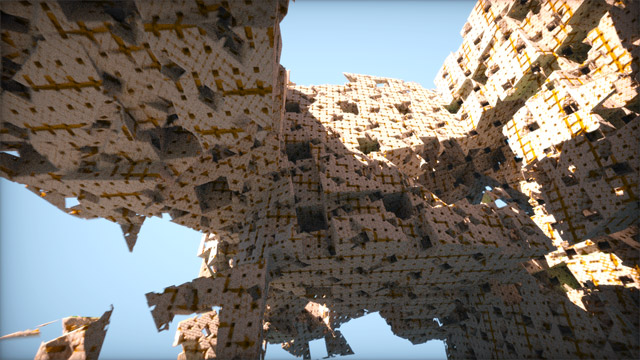
\includegraphics[scale=0.36]{images/cover}
}
\subtitle{}
\author[Dr. Johannes Riesterer] % (optional, for multiple authors)
{Dr.  rer. nat. Johannes Riesterer}

\date[KPT 2004] % (optional)
{}

\subject{Computergrafik}

\frame{\titlepage}


\begin{frame}
    \frametitle{Kameraprojektion}
\framesubtitle{}
    \begin{block}{}
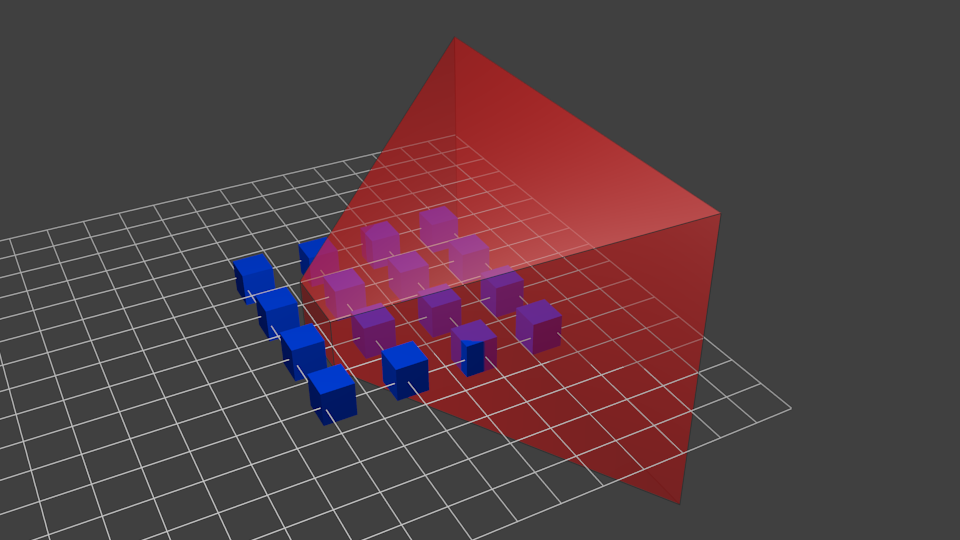
\includegraphics[scale=0.16]{images/nondeforme}
 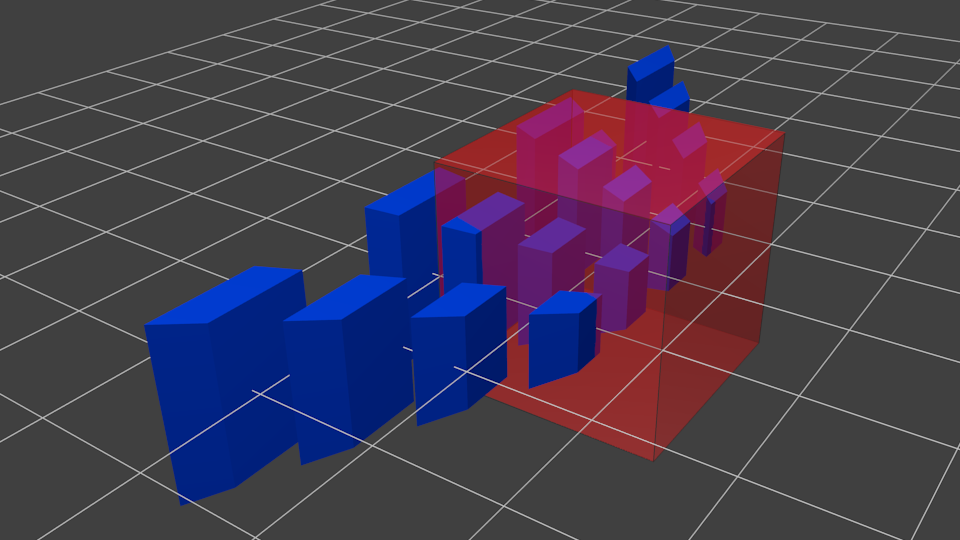
\includegraphics[scale=0.16]{images/deform}
\end{block}
\end{frame}


\begin{frame}
    \frametitle{ Shaderprogramm}
\framesubtitle{}
    \begin{block}{}
\begin{center}
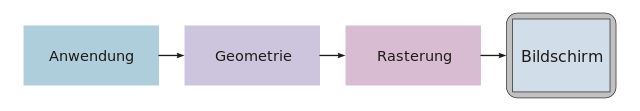
\includegraphics[scale=0.26]{images/cgpipeline_grob}
\end{center}
\end{block}
    \begin{block}{}
\begin{center}
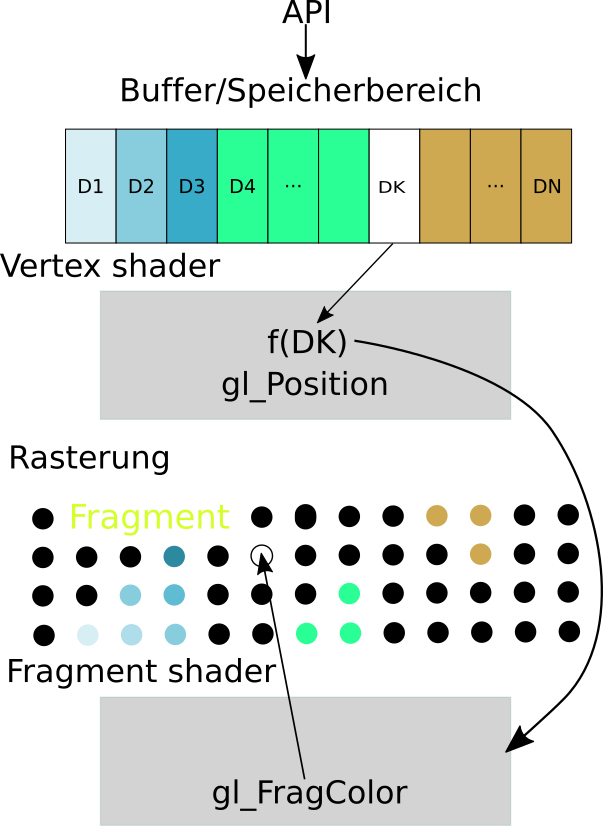
\includegraphics[scale=0.20]{images/Zeichnung_Shaderpipeline}
\end{center}
\end{block}
\end{frame}


\begin{frame}
    \frametitle{OpenGL Pipeline}
\framesubtitle{}
    \begin{block}{}
\begin{center}
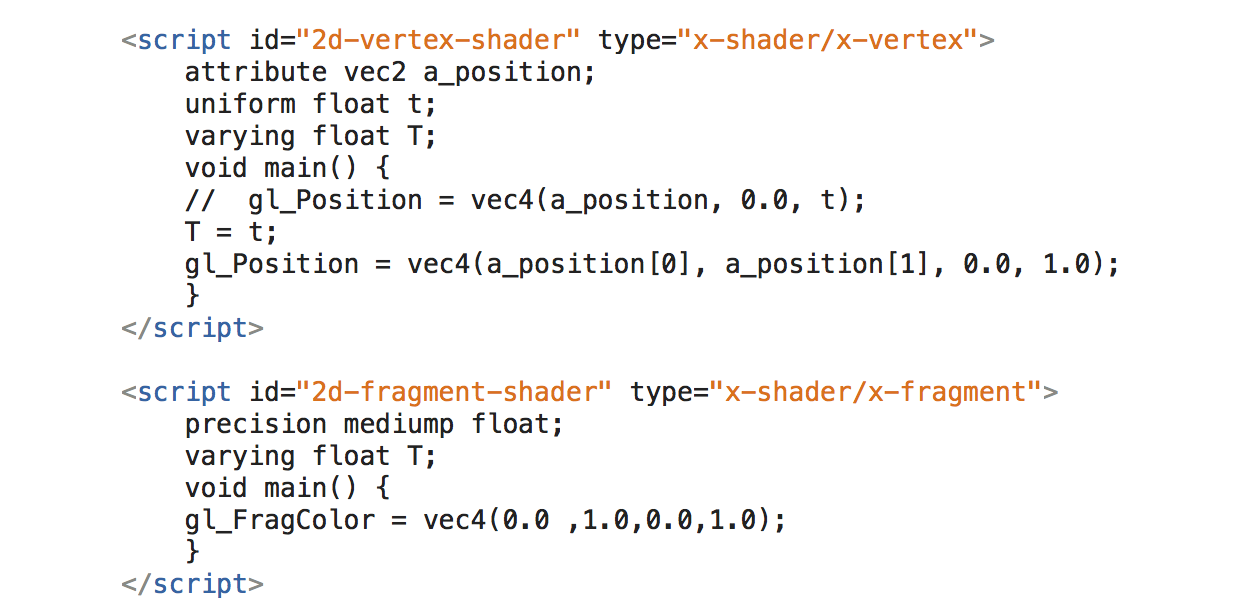
\includegraphics[scale=0.56]{images/shader}
\end{center}
\end{block}
\end{frame}

\begin{frame}
    \frametitle{Basis}
\framesubtitle{}
    \begin{block}{Basis}
Sind $b_1, b_2, b_3$ einer unabhängig, dann heisst die geordnete Menge
$ B = \{ b_1 , b_2, b_3\}$ Basis des $\mathbb{R}^3$.
\end{block}
 \begin{block}{Basisdarstellung}
Für $v \in \mathbb{R}^3$ heisst
\begin{eqnarray*}
& \theta_B : \mathbb{R}^3 \to  \mathbb{R}^3 \\
& \theta_B(v) =  \begin{pmatrix}
 \lambda_1 \\ \lambda_2 \\ \lambda_3
\end{pmatrix}  \\
& \text{mit } \lambda_1 \cdot b_1 + \lambda_2 \cdot b_2  + \lambda_3 \cdot b_3 = v 
\end{eqnarray*}
Darstellung von $v$ bezüglich der Basis $B$.
\end{block}

\end{frame}

\begin{frame}
    \frametitle{Basiswechsel}
\framesubtitle{}
\begin{block}{Basiswechsel berechnen}
\begin{eqnarray*}
& \theta_B(v) =  M_B^{-1} \cdot v, \; \; M_B :=  \begin{pmatrix}
 b_1 & b_2 &  b_3
\end{pmatrix} \text{(column major)}
\end{eqnarray*}
\end{block}

\begin{block}{Basiswechsel}
Seien $B:= \{ b_1, \hdots , b_n \}$ und $B':= \{ b'_1, \hdots , b'_n \}$ zwei Basen des $\mathbb{R}^n$.
Dann heißt $M_{B}^{B'} : = M_{B'}  \cdot M_{B}^{-1} $ die Basiswechselmatrix von $B$ nach $B'$. Wir haben also folgende Situation:
\begin{align*}
\xymatrix{
\mathbb{R}^n  \ar[d]^{I_n} &  & \ar[ll]^{M_B^{-1}} \mathbb{R}^n \ar[d]^{M_{B}^{B'}} \\
\mathbb{R}^n  \ar[rr]^{M_{B'}} & &  \mathbb{R}^n
}
\end{align*}
\end{block}
\end{frame}


\begin{frame}
    \frametitle{Skalarprodukt}
\framesubtitle{}
\begin{block}{Skalarproduktt}
$\langle v ,w \rangle := v^t \cdot w = \sum_{i=1}^{3} v_i \cdot w_i$ \\
Zwei vom Nullvektor verschiedene Vektoren $u,v \in \mathbb{R}^n$ heißen orthogonal, falls $<u,v> = 0$ ist. 
\end{block}
\begin{block}{Norm}
$||v || : = \sqrt{\langle v ,v \rangle} := v^t \cdot w = \sqrt{\sum_{i=1}^{3} v_i ^{2}}$ \\
Ein Vektor $v$ heißt normal, falls $||v|| = 1$ ist.
Ist $w$ ein beliebiger Vektor, so heißt $\frac{1}{||w||} w$ die Normalisierung von $w$, denn er ist normal.
\end{block}
\begin{block}{Satz}
Für den von zwei Vektoren $u,v$ eingeschlossenen Winkel $\varphi$ gilt:
\begin{align*}
\cos(\varphi) = \frac{<u,v>}{||u|| \cdot ||v||}
\end{align*}
\end{block}
\end{frame}


\begin{frame}
    \frametitle{Kreuzprodukt}
\framesubtitle{}
\begin{block}{Kreuzprodukt}
Für $u = \begin{pmatrix} u_1 \\ u_2 \\ u_3 \end{pmatrix}$ und $v= \begin{pmatrix} v_1 \\ v_2 \\ v_3 \end{pmatrix}$ heißt
\begin{align*}
u \times v :=  \begin{pmatrix} u_2 v_3 - u_3v_2  \\ u_3 v_1 - u_1v_3 \\ u_1 v_2 - u_2 v_1\end{pmatrix} 
\end{align*}
das Kreuzprodukt von $u$ und $v$.
Es gilt
\begin{itemize}
\item $<u \times v, u> =  <u \times v, v> = 0$ 
\item $u \times v = - (v \times u)$
\item $u \times v = 0$ genau dann, wenn $u$ und $v$ linear abhängig sind.
\end{itemize}
\end{block}
\end{frame}

\begin{frame}
    \frametitle{Orthonormalbasis}
\framesubtitle{}
\begin{block}{Orthonormalbasis}
Eine Basis  $B:= \{ b_1, b_2 , b_3 \}$ heißt Orthonormalbasis (kurz ONB), falls 
\begin{align*}
<b_i, b_j> = \begin{cases}  1 \; \text{falls }  i = j  \\ 0 \; \text{sonst}\end{cases}
\end{align*}
gilt. Insbesondere sind alle $b_i$ normal.
\end{block}
\end{frame}


\begin{frame}
    \frametitle{Orthonormalbasis}
\framesubtitle{}
\begin{block}{Basis-Wechsel-Matrix}
Ist  $B:= \{ b_1, \hdots , b_n \}$  eine ONB, so gilt
\begin{align*}
M_{B}^{-1} = M_{B}^t
\end{align*}
\end{block}
\begin{block}{Drehungen}
Eine Matrix $O \in \mathbb{M}^{n \times n}$ heißt orthogonal, falls
$O^{-1} = O^t$ ist.  Sie ist genau dann  orthogonal, falls
\begin{align*}
\det(O) \in  \{-1, 1 \} \; .
\end{align*}
Ist $\det(O) = 1$, so nennen wir $O$ eine Drehung und 
$SO(n) := \{ O \in \mathbb{M}^{n \times n} | \det(O) = 1\}$ die Drehgruppe (oder auch spezielle orthogonale Gruppe).
\end{block}

\end{frame}


\begin{frame}
    \frametitle{Orthonormalbasis}
\framesubtitle{}
\begin{block}{Basis-Wechsel-Matrix}
Sei $O \in \mathbb{M}^{n \times n}$ eine orthogonale Matrix, dann gilt für alles $v,w \in \mathbb{R}^n$
\begin{align*}
< O \cdot v \; , \;  O \cdot w > = <v \; , \; w>
\end{align*}
und somit insbesondere 
\begin{align*}
|| O \cdot v|| = ||v|| \; .
\end{align*}
\end{block}

\end{frame}


\begin{frame}
    \frametitle{Orthonormalbasis}
\framesubtitle{}
\begin{block}{Eulerwinkel}
Jede Drehung  $O \in SO(3)$  lässt sich zerlegen in ein Produkt
\begin{align*}
O = 
\begin{pmatrix}
1 & 0 & 0 \\
0 & \cos(\phi) & \pm \sin(\phi) \\ 
 0 & \mp \sin(\phi) & \cos(\phi)
\end{pmatrix}
\cdot
\begin{pmatrix}
 \cos(\psi) & 0 &   \sin(\psi) \\ 
0 & 1 & 0 \\ 
- \sin(\psi) & 0& \cos(\psi)
\end{pmatrix} \\
\cdot \begin{pmatrix}
 \cos(\xi) &  \sin(\xi)  & 0\\ 
 - \sin(\xi) & \cos(\xi) & 0 \\
0 & 0 & 1 
\end{pmatrix} 
\end{align*} 
Die Winkel $\phi, \psi, \xi$ heißen  Eulerwinkel. 
\end{block}

\end{frame}


\begin{frame}
    \frametitle{Orthonormalbasis}
\framesubtitle{}
\begin{block}{Eulerwinkel}
Die  Zerlegung  $O \in SO(3)$  einer Drehung in obiges Produkt ist  nicht eindeutig.
Ein anschauliches Beispiel dafür liefert der sogenannte "Gimbal lock". $SO(3)$ ist also nicht das Produkt von drei Intervallen sondern
es ist $SO(3) = S^{3}/ \{ \pm 1 \}$.

\begin{figure}[H]
    \centering
    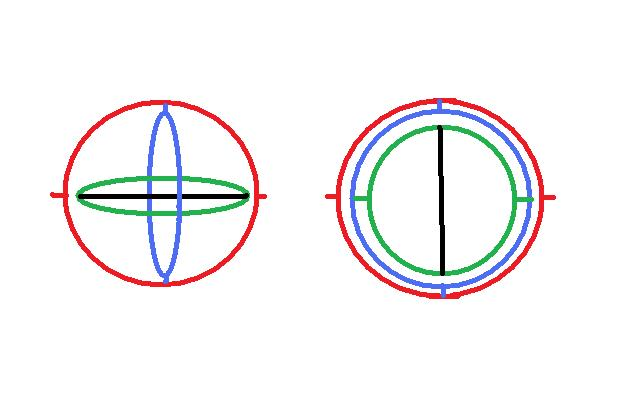
\includegraphics[width=0.9\textwidth]{images/gimbalLock.jpg}
    \caption{Kardansche Aufhängung und Gimbal lock}
    \label{fig:gimbal+lock}
\end{figure}

\end{block}

\end{frame}


\begin{frame}
    \frametitle{Affiner Raum}
\framesubtitle{}
\begin{block}{Affiner Raum}
Der Affine Raum $\mathbb{A}^3$ ist ein Tupel $\bigl( \mathbb{R}^3, (\mathbb{R}^3, + , \cdot ) \bigr )$
zusammen mit den Abbildung 
\begin{align*}
\text{---} : \mathbb{R}^3 \times \mathbb{R}^3  & \to (\mathbb{R}^3, + , \cdot ) \\
\overline{PQ} & := Q-P  
\end{align*}
und
\begin{align*}
+ : \mathbb{R}^n \times (\mathbb{R}^3, + , \cdot )   & \to  \mathbb{R}^3\\
\begin{pmatrix}
P_1 \\ \vdots \\ P_3
\end{pmatrix} + \begin{pmatrix}
v_1 \\ \vdots \\ v_3
\end{pmatrix} & := \begin{pmatrix}
P_1  + v_1 \\ \vdots \\ P_3 + v_3
\end{pmatrix}   \;.
\end{align*}

\end{block}

\end{frame}


\begin{frame}
    \frametitle{Affiner Raum}
\framesubtitle{}
\begin{block}{Affiner Raum}
Die Elemente (Vektoren) aus $\mathbb{R}^3$ nennt man auch  Punkte in Abgrenzung zu den Vektoren aus $(\mathbb{R}^3, + , \cdot )$.  
Für Punkte $P,Q \in \mathbb{R}^3$ ist also $\overline{PQ}$ ein Vektor, auch Verbindungsvektor genannt.
\end{block}

\end{frame}


\begin{frame}
    \frametitle{Affiner Raum}
\framesubtitle{}
\begin{block}{Affine basis}
Ist $B:= \{b_1, b_2 , b_3 \}$ eine Basis des Vektorraums  $(\mathbb{R}^3, + , \cdot )$ und $P \in \mathbb{A}$ ein Punkt, so nennen wir das Tupel
$(P, B)$ eine affine Basis. Für jeden Punkt $Q$ gibt es dann also Skalare $\lambda_1,\hdots ,\lambda_n$ mit 
\begin{align*}
Q = P + \sum_{i=1}^{3} \lambda_i \cdot b_i  \; .
\end{align*}
Der Punkt $\theta_{(P,B)}(Q):= \begin{pmatrix}  \lambda_1 \\   \lambda_2 \\  \lambda_3 \end{pmatrix}$ heißt die Darstellung von $Q$ bezüglich der affinen Basis $(P,B)$. 
\end{block}

\end{frame}



\begin{frame}
    \frametitle{Affiner Raum}
\framesubtitle{}
\begin{block}{Affine Abbildung}
Abbildungen der Form
\begin{align*}
\phi &: \mathbb{A}^3 \to \mathbb{A}^3 \\
\phi(P) & := A \cdot P + t
\end{align*} 
mit $A \in M^{3 \times 3}$ und $t \in (\mathbb{R}^3, + , \cdot )$ heißen affine Abbildungen.
Insbesondere heißt eine affine Abbildung mit $A = I_3$ und $t \neq 0$ Translation.
\end{block}
\begin{block}{Abstand}
Der Abstand von  $P,Q \in \mathbb{A}$  ist definiert durch
\begin{align*}
d : \mathbb{A}^3 \times \mathbb{A}^3 \to \mathbb{R} \\
d(P,Q) := || \overline{PQ} || \; .
\end{align*}
\end{block}

\end{frame}



\begin{frame}
    \frametitle{Affiner Raum}
\framesubtitle{}
\begin{block}{Affiner Basiswechsel}

Sind $(P,B:= \{b_1, \hdots , b_n \})$  und $(P',B':= \{b'_1, \hdots , b'_n \})$ zwei affine Basen  und definieren wir 
die Abbildung
\begin{align*}
\theta_{(P,B)} & :  \mathbb{A}^n \to \mathbb{A}^n \\
\theta_{(P,B)}(Q) & := M_B \cdot Q - M_B \cdot P \; ,
\end{align*}
so erhalten wir analog zu der Situation in Vektorräumen
\begin{align*}
\xymatrix{
\mathbb{A}^n  \ar[d]^{\text{id}} &  & \ar[ll]^{\theta_{(P,B)}^{-1}} \mathbb{A}^n \ar[d]^{\theta_{(P,B)}^{(P',B')}} \\
\mathbb{A}^n  \ar[rr]^{\theta_{(P',B')}} & &  \mathbb{A}^n
}
\end{align*}
mit $\theta_{(P,B)}^{(P',B')} (Q) :=   \theta_{(P',B')} \biggl ( \theta_{(P,B)}^{-1} (Q) \biggr)$.
\end{block}

\end{frame}



\begin{frame}
    \frametitle{Homogene Koordinaten}
\framesubtitle{}
\begin{block}{Projektier Raum}

Der projektive  Raum ist definiert als
\begin{align*}
\mathbb{P}^3 := \mathbb{R}^{4} - \{ 0\} / \sim \\
v \sim w \Leftrightarrow v = \lambda w \text{ für ein } \lambda \neq 0 \in \mathbb{R} \; . 
\end{align*}
\end{block}
\end{frame}

\begin{frame}
    \frametitle{Homogene Koordinaten}
\framesubtitle{}
\begin{block}{Homogene Koordinaten}
Wir haben die Abbildung
\begin{align*}
\mathbb{A}^3 & \to \mathbb{P}^3 \\
\begin{pmatrix} p_1 \\ p_2 \\ p_3 \end{pmatrix} & \mapsto \begin{pmatrix} p_1 \\ p_2 \\ p_3  \\  1\end{pmatrix} 
\end{align*}
und nennen das Bild eines Punktes unter dieser Abbildung die homogenen Koordinaten.
\end{block}
\end{frame}

\begin{frame}
    \frametitle{Homogene Koordinaten}
\framesubtitle{}
\begin{block}{Homogene Koordinaten}
Auf der Menge der homogenen Koordinaten haben wir die Umkehrabbildung
\begin{align*}
& \mathbb{P}^3 - \Biggl \{\begin{pmatrix} p_1 \\ p_2 \\ p_3  \\ p_4 \end{pmatrix}\Bigg | \; p_{4} = 0 \Biggr \}   \to \mathbb{A}^3 \\
& \begin{pmatrix} p_1 \\ p_2 \\ p_3  \\  p_{4} \end{pmatrix}   \mapsto \begin{pmatrix}  \frac{p_1}{ p_{4}} \\ \frac{p_2}{ p_{4}}  \\ \frac{p_3}{ p_{4}}  \end{pmatrix}  \; .
\end{align*}
\end{block}
\end{frame}


\begin{frame}
    \frametitle{Homogene Koordinaten}
\framesubtitle{}
\begin{block}{Homogene Koordinaten}
Die Punkte $ \Biggl \{ \begin{pmatrix} p_1 \\ p_2 \\ p_3  \\ 0 \end{pmatrix} \Biggr \} $ heissen unendlich ferne Punkte.

\begin{align*}
 \begin{pmatrix} p_1 \\ p_2 \\ \vdots  \\ 0 \end{pmatrix}  =\lim_{n \to \infty} \begin{pmatrix} p_1 \\ p_2 \\ \vdots  \\ \frac{1}{n} \end{pmatrix}  \cong  \lim_{n \to \infty} n \cdot  \begin{pmatrix} p_1 \\ p_2 \\ p_3 \end{pmatrix} 
\end{align*}
\end{block}

\begin{block}{Zerlegung des projektiven Raum}
Der projektive Raum ist damit die Vereinigung des Affinen Raumes und den unendlich fernen Punkten. "Parallelen schneiden sich in den unendlich fernen Punkten".
\end{block}
\end{frame}

\begin{frame}
    \frametitle{Homogene Koordinaten}
\framesubtitle{}
\begin{block}{Projektive Abbildungen}
Die Matrizenmultiplikation
\begin{align*}
\mathbb{R}^{4} \to \mathbb{R}^{4} \\
v \mapsto A \cdot v
\end{align*}
setzt sich wegen der Eigenschaft $A \cdot (\lambda v) = \lambda A \cdot v$ zu einer Abbildung
\begin{align*}
\mathbb{P}^{3} \to \mathbb{P}^{3} \\
p \mapsto A \cdot p
\end{align*}
fort. 
\end{block}
\end{frame}

\begin{frame}
    \frametitle{Homogene Koordinaten}
\framesubtitle{}
\begin{block}{Projektive Abbildungen}
Wir können damit und mit der Definition der Matrix-Vektor-Multiplikation eine affine Abbildung 
\begin{align*}
\phi : \mathbb{A}^{3} \to \mathbb{A}^{3} \\
\phi(v):=  A \cdot v + t
\end{align*}
in homogenen Koordinate ausdrücken durch eine Matrizenmultiplikation
\begin{align*}
\begin{pmatrix} v \\ 1\end{pmatrix} \mapsto \begin{pmatrix}  A  & t  \\ 0 &1\end{pmatrix} \cdot  \begin{pmatrix} v \\ 1\end{pmatrix}   \; .
\end{align*}
\end{block}
\end{frame}

Definieren wir die Matrizen
\begin{align*}
K_{persp_{xy}} := \begin{pmatrix}  
1   &  0 & 0 & 0  \\
0   &  1 & 0 & 0  \\
0   &  0 & 1 & 0  \\
0   &  0 & \frac{1}{d} & 1  
\end{pmatrix} ,
K_{orth_{xy}} := \begin{pmatrix}  
1   &  0 & 0 & 0  \\
0   &  1 & 0 & 0  \\
0   &  0 & 0 & 1  
\end{pmatrix} \; ,
\end{align*}


so können wir die Zentralprojektion auf die $X-Y$-Ebene mit Augendistanz $d$ durch die Hintereinanderausführung folgender Abbildungen darstellen:
\begin{align*}
& persp_{xy} :\mathbb{R}^3   \to \mathbb{A}^3    \to  \mathbb{A}^3    \to \mathbb{A}^2    \to \mathbb{R}^2  \\
&\begin{pmatrix} x \\ y \\ z \end{pmatrix} \mapsto \begin{pmatrix} x \\ y \\ z \\ 1 \end{pmatrix}   \mapsto K_{persp_{xy}} \cdot  \begin{pmatrix} x \\ y \\ z \\ 1 \end{pmatrix} =   \begin{pmatrix} x \\ y \\ z \\ \frac{z}{d} + 1 \end{pmatrix} \\
 & \mapsto K_{orth_{xy}} \cdot   \begin{pmatrix} x \\ y \\ z \\ \frac{z}{d} + 1 \end{pmatrix}=   \begin{pmatrix} x \\ y \\ \frac{z}{d} + 1 \end{pmatrix}   \mapsto 
 \begin{pmatrix}  \frac{x}{\frac{z}{d} +1 } \\   \frac{y}{\frac{z}{d} +1 } \end{pmatrix}
 \end{align*}



\end{document}
